\documentclass[11pt,letterpaper]{article}
\usepackage{../../assets/scientific_report}
\usepackage{amsmath}
\usepackage{float}
\usepackage{listings}
\usepackage{xcolor}
\usepackage{graphicx}
\usepackage{geometry}
\geometry{headheight=23pt, top=2cm, bottom=2cm, left=2.5cm, right=2.5cm}
\setlength{\parskip}{0.5em}
\setlength{\parindent}{0pt}
\lstset{
  language=C,
  basicstyle=\ttfamily\small,
  keywordstyle=\color{blue}\bfseries,
  commentstyle=\color{green!60!black}\itshape,
  stringstyle=\color{red!80!black},
  numbers=left,
  numberstyle=\tiny\color{gray},
  numbersep=8pt,
  frame=single,
  breaklines=true,
  captionpos=b,
  tabsize=4,
  showstringspaces=false,
  inputencoding=utf8,
  extendedchars=true,
  literate={ã}{{\~a}}1 {õ}{{\~o}}1 {á}{{\'a}}1 {à}{{\`a}}1 {â}{{\^a}}1 {é}{{\'e}}1 {ê}{{\^e}}1 {í}{{\'i}}1 {ó}{{\'o}}1 {ô}{{\^o}}1 {ú}{{\'u}}1 {ç}{{\c{c}}}1 {Ã}{{\~A}}1 {Õ}{{\~O}}1 {Á}{{\'A}}1 {É}{{\'E}}1 {Í}{{\'I}}1 {Ó}{{\'O}}1 {Ô}{{\^O}}1 {Ú}{{\'U}}1 {Ç}{{\c{C}}}1 {—}{{---}}1
}
\begin{document}
\pagestyle{plain}
\begin{center}
{\LARGE\bfseries Difusão viscosa 2D: particionamento e balanceamento de carga}\\[0.4em]
{\normalsize Eugenio Vitor Lopes dos Santos}\\[0.3em]
{\small DCA3703, Programação Paralela, Universidade Federal do Rio Grande do Norte}\\[0.3em]
\end{center}
\section{Enunciado}
\begin{quote}
``Escreva um código que simule o movimento de um fluido ao longo do tempo usando a equação de Navier-Stokes, considerando apenas os efeitos da viscosidade. Desconsidere a pressão e quaisquer forças externas. Utilize diferenças finitas para discretizar o espaço e simule a evolução da velocidade do fluido no tempo. Inicialize o fluido parado ou com velocidade constante e verifique se o campo permanece estável. Em seguida, crie uma pequena perturbação e observe se ela se difunde suavemente. Após validar o código, paralelize-o com OpenMP e explore o impacto das cláusulas \texttt{schedule} e \texttt{collapse} no desempenho da execução paralela.''
\end{quote}

\section{Fundamentação teórica}

\subsection{Difusão viscosa e diferenças finitas}
Considerando apenas a viscosidade, foi adotada a equação de difusão para uma componente escalar da velocidade:
\[
\frac{\partial u}{\partial t}=\nu\nabla^2u,
\]
em que $u$ representa a componente de velocidade e $\nu$ é a viscosidade cinemática. Nessa simplificação, foram omitidas a advecção, a pressão e as forças externas. Portanto, o programa não resolve o sistema completo de Navier--Stokes incompressível.

A discretização utiliza Euler explícito no tempo e diferenças centrais no espaço, formando o esquema FTCS. Para uma malha quadrada de espaçamento $h$:
\[
u^{n+1}_{i,j}=u^n_{i,j}+r\left(u^n_{i-1,j}+u^n_{i+1,j}+u^n_{i,j-1}+u^n_{i,j+1}-4u^n_{i,j}\right),
\qquad r=\frac{\nu\Delta t}{h^2}.
\]
Esse stencil de cinco pontos calcula o novo valor a partir da célula central e de seus quatro vizinhos no instante anterior. Foram utilizados $\nu=0{,}1$, $\Delta t=0{,}2$ e $h=1$, resultando em $r=0{,}02$. A condição de estabilidade em duas dimensões é $0\le r\le1/4$, atendida pelos parâmetros utilizados.

Em um campo constante, o laplaciano discreto é zero e o valor permanece inalterado, desde que as bordas tenham o mesmo valor. Em uma perturbação localizada, a difusão reduz o pico e espalha o campo para as células vizinhas.

\subsection{Particionamento e políticas de escalonamento}
A diretiva \texttt{parallel} cria a equipe de threads, enquanto \texttt{omp for} distribui as iterações entre elas. A cláusula \texttt{schedule} define essa distribuição:
\begin{itemize}
\item \texttt{static}: divide as iterações em blocos aproximadamente iguais. Sem chunk explícito, cada thread recebe no máximo um bloco. Apresenta baixo custo de gerenciamento e é adequado para trabalho uniforme.
\item \texttt{dynamic,k}: distribui blocos de $k$ iterações conforme as threads terminam os anteriores. Pode reduzir o desbalanceamento, mas exige gerenciamento a cada bloco.
\item \texttt{guided,k}: também entrega novos blocos conforme a conclusão do trabalho, porém começa com blocos maiores e reduz seus tamanhos. O valor $k$ é o mínimo, exceto no último bloco.
\end{itemize}
O chunk conta iterações do laço distribuído. Blocos pequenos aumentam as oportunidades de balanceamento e o custo de distribuição; blocos grandes reduzem esse custo, mas deixam menos trabalho disponível para redistribuir. Nesta tarefa, todas as células internas executam a mesma operação.

\subsection{Efeito de \texttt{collapse(2)}}
Sem \texttt{collapse}, apenas o laço externo é distribuído: cada iteração corresponde a uma linha. Com \texttt{collapse(2)}, os laços de $i$ e $j$ formam um único espaço de iterações, no qual cada unidade corresponde a uma célula.

Para $N=512$, são 510 linhas ou $510^2=260.100$ células internas. Assim, chunk 16 representa 16 linhas sem \texttt{collapse} e 16 células com a cláusula. Essa diferença precisa ser considerada na comparação de desempenho. O laço temporal permanece sequencial, pois cada passo depende do campo produzido pelo anterior.

\section{Implementação}
\subsection{Organização das versões}
Foram implementadas sete versões independentes em C11: uma referência sequencial e seis variantes OpenMP. Cada arquivo contém a inicialização, a atualização do campo, a medição de tempo e a exportação. A separação facilita a comparação das alterações nos pragmas.

A malha tem $512\times512$ pontos e são realizados 500 passos. Esses valores são definidos no código por \texttt{tamanho\_grid} e \texttt{num\_passos\_tempo}. A interface recebe \texttt{[modo [arquivo-campo]]}: modo 0 para a perturbação gaussiana, modo 1 para o campo nulo e modo 2 para o campo unitário. O modo padrão é 0. São verificados os argumentos, as alocações e a escrita do arquivo.

A gaussiana tem amplitude 0,1, centro na malha e $\sigma=N/10$. As bordas são fixas: zero nos modos 0 e 1, e um no modo 2. Dois vetores de \texttt{double}, acessados por \texttt{c = i*N+j}, armazenam os campos. As bordas são inicializadas nos dois vetores e ficam fora dos laços de atualização.

\begin{table}[H]
\centering
\begin{tabular}{lll}
\hline
Versão & Política & Unidade distribuída \\
\hline
v0 & Sequencial & Sem distribuição \\
v1 & \texttt{static} & Linha \\
v2 & \texttt{static}, \texttt{collapse(2)} & Célula \\
v3 & \texttt{dynamic,16} & Bloco de 16 linhas \\
v4 & \texttt{dynamic,16}, \texttt{collapse(2)} & Bloco de 16 células \\
v5 & \texttt{guided,16}, \texttt{collapse(2)} & Bloco decrescente de células \\
v6 & \texttt{guided,16} & Bloco decrescente de linhas \\
\hline
\end{tabular}
\caption{Versões completas e independentes. Em guided, 16 é o tamanho mínimo, salvo o último bloco.}
\end{table}
\subsection{Atualização do campo e sincronização}
O vetor apontado por \texttt{u} contém o campo atual; o vetor apontado por \texttt{v} recebe o próximo campo. Eles representam dois instantes da mesma componente de velocidade. Em cada passo, as threads leem apenas \texttt{u} e escrevem em posições distintas de \texttt{v}. Atualizar o próprio \texttt{u} misturaria valores de instantes diferentes e introduziria dependências entre as iterações.

Uma única região \texttt{parallel} envolve os 500 passos. Dentro dela, cada thread percorre o laço temporal com seu contador local, e \texttt{omp for} divide as atualizações espaciais. O trecho abaixo mostra a versão v1; as demais variantes paralelas alteram a política e a presença de \texttt{collapse(2)}.

\lstinputlisting[firstline=68,lastline=80,firstnumber=68,gobble=8,caption={Laço temporal e troca de buffers na versão v1.},label={lst:atualizacao}]{../v1_static.c}

A barreira implícita ao final de \texttt{omp for} garante que todas as células foram atualizadas antes da troca. A diretiva \texttt{single} permite que uma thread troque os ponteiros, sem copiar a matriz. Sua barreira final garante que o próximo passo comece com os ponteiros já trocados. Portanto, retirar qualquer uma dessas barreiras com \texttt{nowait}, mantendo o restante do código, comprometeria a correção. Não é necessário usar \texttt{critical} ou \texttt{atomic} por célula, pois cada posição de saída tem um único escritor.

Foi utilizado \texttt{default(none)} para explicitar o compartilhamento das variáveis sem escopo predeterminado. Os ponteiros \texttt{u} e \texttt{v}, os parâmetros e o registro de threads são compartilhados. Os contadores locais e as variáveis \texttt{c} e \texttt{tmp} são privados. O número efetivo de threads é obtido com \texttt{omp\_get\_num\_threads()} dentro de um \texttt{single} inicial.

\subsection{Compilação e execução}
A compilação utiliza GCC com otimização \texttt{-O2}, avisos habilitados e \texttt{-fopenmp} apenas nas variantes paralelas. Os exemplos abaixo são executados no diretório \texttt{tarefa11/}:
\begin{lstlisting}[language=bash,caption={Compilação, validação e execução.}]
gcc -std=c11 -O2 -Wall -Wextra v0_seq.c -lm -o ns_v0
gcc -std=c11 -O2 -Wall -Wextra -fopenmp v1_static.c -lm -o ns_v1
bash test.sh
./ns_v0 1
./ns_v0 2
OMP_NUM_THREADS=4 ./ns_v1 0 campo.txt
\end{lstlisting}
Nas versões \texttt{dynamic} e \texttt{guided}, a macro \texttt{CHUNK\_SIZE} vale 16 por padrão e pode ser alterada na compilação com \texttt{-DCHUNK\_SIZE=valor}. Essa opção foi utilizada no estudo de chunks equivalentes.

\section{Resultados}
\subsection{Validação numérica}
O script \texttt{test.sh} compila as sete versões com \texttt{-std=c11 -O2 -Wall -Wextra -Werror}, acrescentando \texttt{-fopenmp} às paralelas e \texttt{-lm} na ligação. Foram aprovadas 30 comparações exatas dos campos completos de $512\times512$ pontos: para cada variante paralela, o modo gaussiano foi testado com 1, 2 e 4 threads; os modos nulo e unitário, com quatro threads.

O campo parado permaneceu nulo e o campo constante permaneceu unitário. As versões paralelas produziram os mesmos campos da referência sequencial. Também foram verificadas a não negatividade do campo perturbado, seu pico abaixo de 0,1 e a rejeição de argumentos inválidos e de um caminho de saída inexistente.

A Figura~\ref{fig:difusao} compara a gaussiana inicial com o campo após 500 passos. A redução do pico e o aumento do raio quadrático médio indicam o espalhamento da perturbação. Esses testes verificam os casos executados; a estabilidade do esquema decorre também da condição sobre $r$ apresentada na fundamentação.

\begin{figure}[H]
\centering
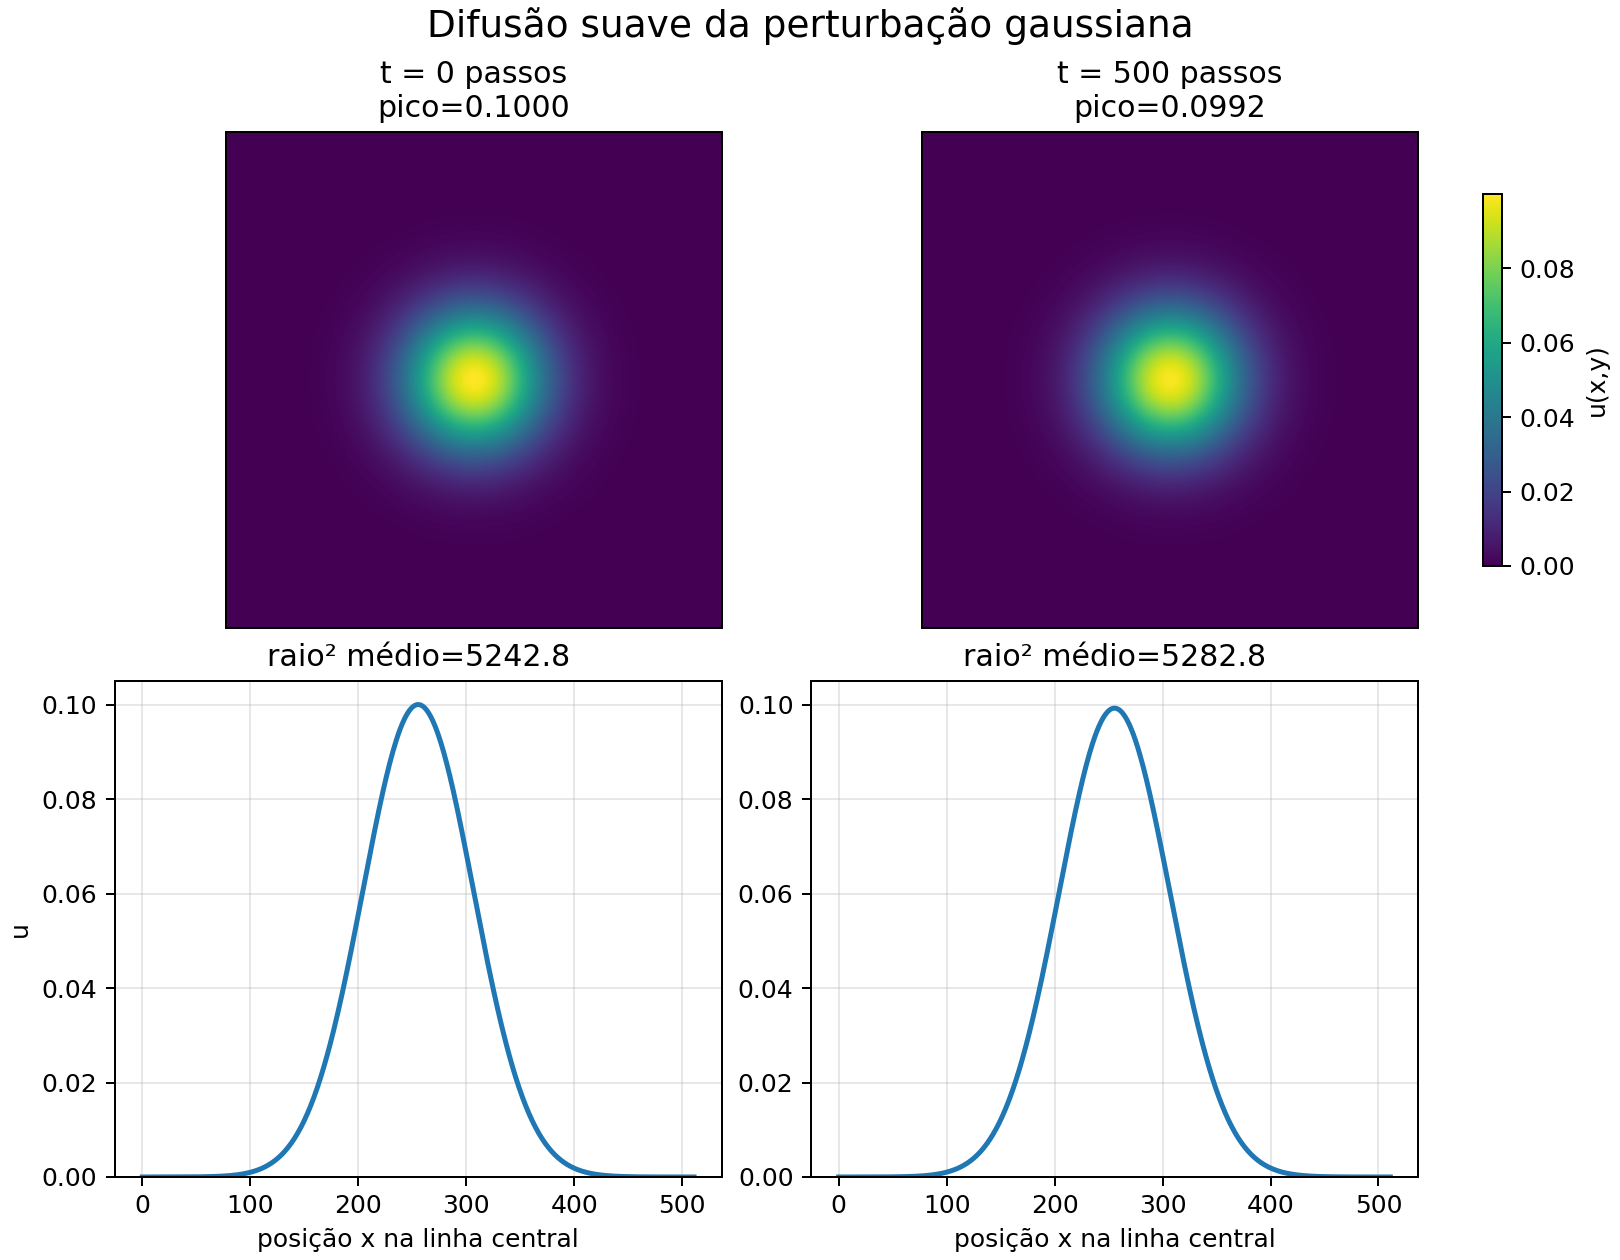
\includegraphics[width=0.95\textwidth]{../visualizacao_difusao.png}
\caption{Difusão da perturbação gaussiana no início e após 500 passos.}
\label{fig:difusao}
\end{figure}
\subsection{Medição de desempenho}
O benchmark foi executado com GCC 13.3.0 no Intel Core i7-14700HX sob WSL2, usando uma grade $512\times512$, 500 passos e uma varredura de 1 a 28 threads. Esse é o número de processadores lógicos disponíveis no ambiente virtualizado. Cada ponto de 1 a 25 threads usa a mediana de cinco repetições após aquecimento. Como a primeira varredura apresentou picos abruptos no final, os pontos de 26 a 28 threads foram repetidos dez vezes sob as mesmas condições e substituídos por essas medianas confirmadas. Foram usadas as opções \texttt{-std=c11}, \texttt{-O2}, \texttt{-Wall} e \texttt{-Wextra}, além de \texttt{-lm}; nas variantes paralelas, foi acrescentado \texttt{-fopenmp}. Foram fixados \texttt{OMP\_DYNAMIC=FALSE}, \texttt{OMP\_PROC\_BIND=close} e \texttt{OMP\_PLACES=cores}.

O cronômetro \texttt{CLOCK\_MONOTONIC} cobre a região paralela, o stencil, as barreiras e a troca de ponteiros. Alocação, inicialização, cálculo dos diagnósticos (mínimo, pico e soma) e exportação ficam fora da temporização. A Tabela~\ref{tab:desempenho} apresenta medianas selecionadas; as Figuras~\ref{fig:tempo} e~\ref{fig:speedup} mostram toda a varredura e o speedup $S(p)=T_{seq}/T_p$, em que $T_{seq}$ é o tempo da versão sequencial e $T_p$ é o tempo com $p$ threads. O conjunto consolidado está em \texttt{../runs/resultado-confirmado/}; as duas execuções de origem permanecem preservadas para rastreabilidade.

\begin{table}[H]
\centering
\small
\resizebox{\textwidth}{!}{%
\begin{tabular}{lrrrrrr}
\hline
Versão & 1 thread & 2 threads & 4 threads & 8 threads & 14 threads & 28 threads \\
\hline
v1 static & 0,0970 & 0,0531 & 0,0289 & 0,0223 & 0,0207 & 0,0185 \\
v2 static + collapse & 0,1312 & 0,0722 & 0,0411 & 0,0326 & 0,0280 & 0,0488 \\
v3 dynamic & 0,1064 & 0,0621 & 0,0337 & 0,0220 & 0,0228 & 0,0276 \\
v4 dynamic + collapse & 0,2241 & 0,3662 & 0,3482 & 0,3342 & 0,3007 & 0,3225 \\
v5 guided + collapse & 0,1318 & 0,0706 & 0,0395 & 0,0277 & 0,0242 & 0,0329 \\
v6 guided & 0,1239 & 0,0588 & 0,0327 & 0,0240 & 0,0229 & 0,0269 \\
\hline
\end{tabular}%
}
\caption{Tempo mediano em segundos, selecionado da varredura completa de 1 a 28 threads. A referência sequencial teve mediana de 0,1049 s.}
\label{tab:desempenho}
\end{table}

\begin{figure}[H]
\centering
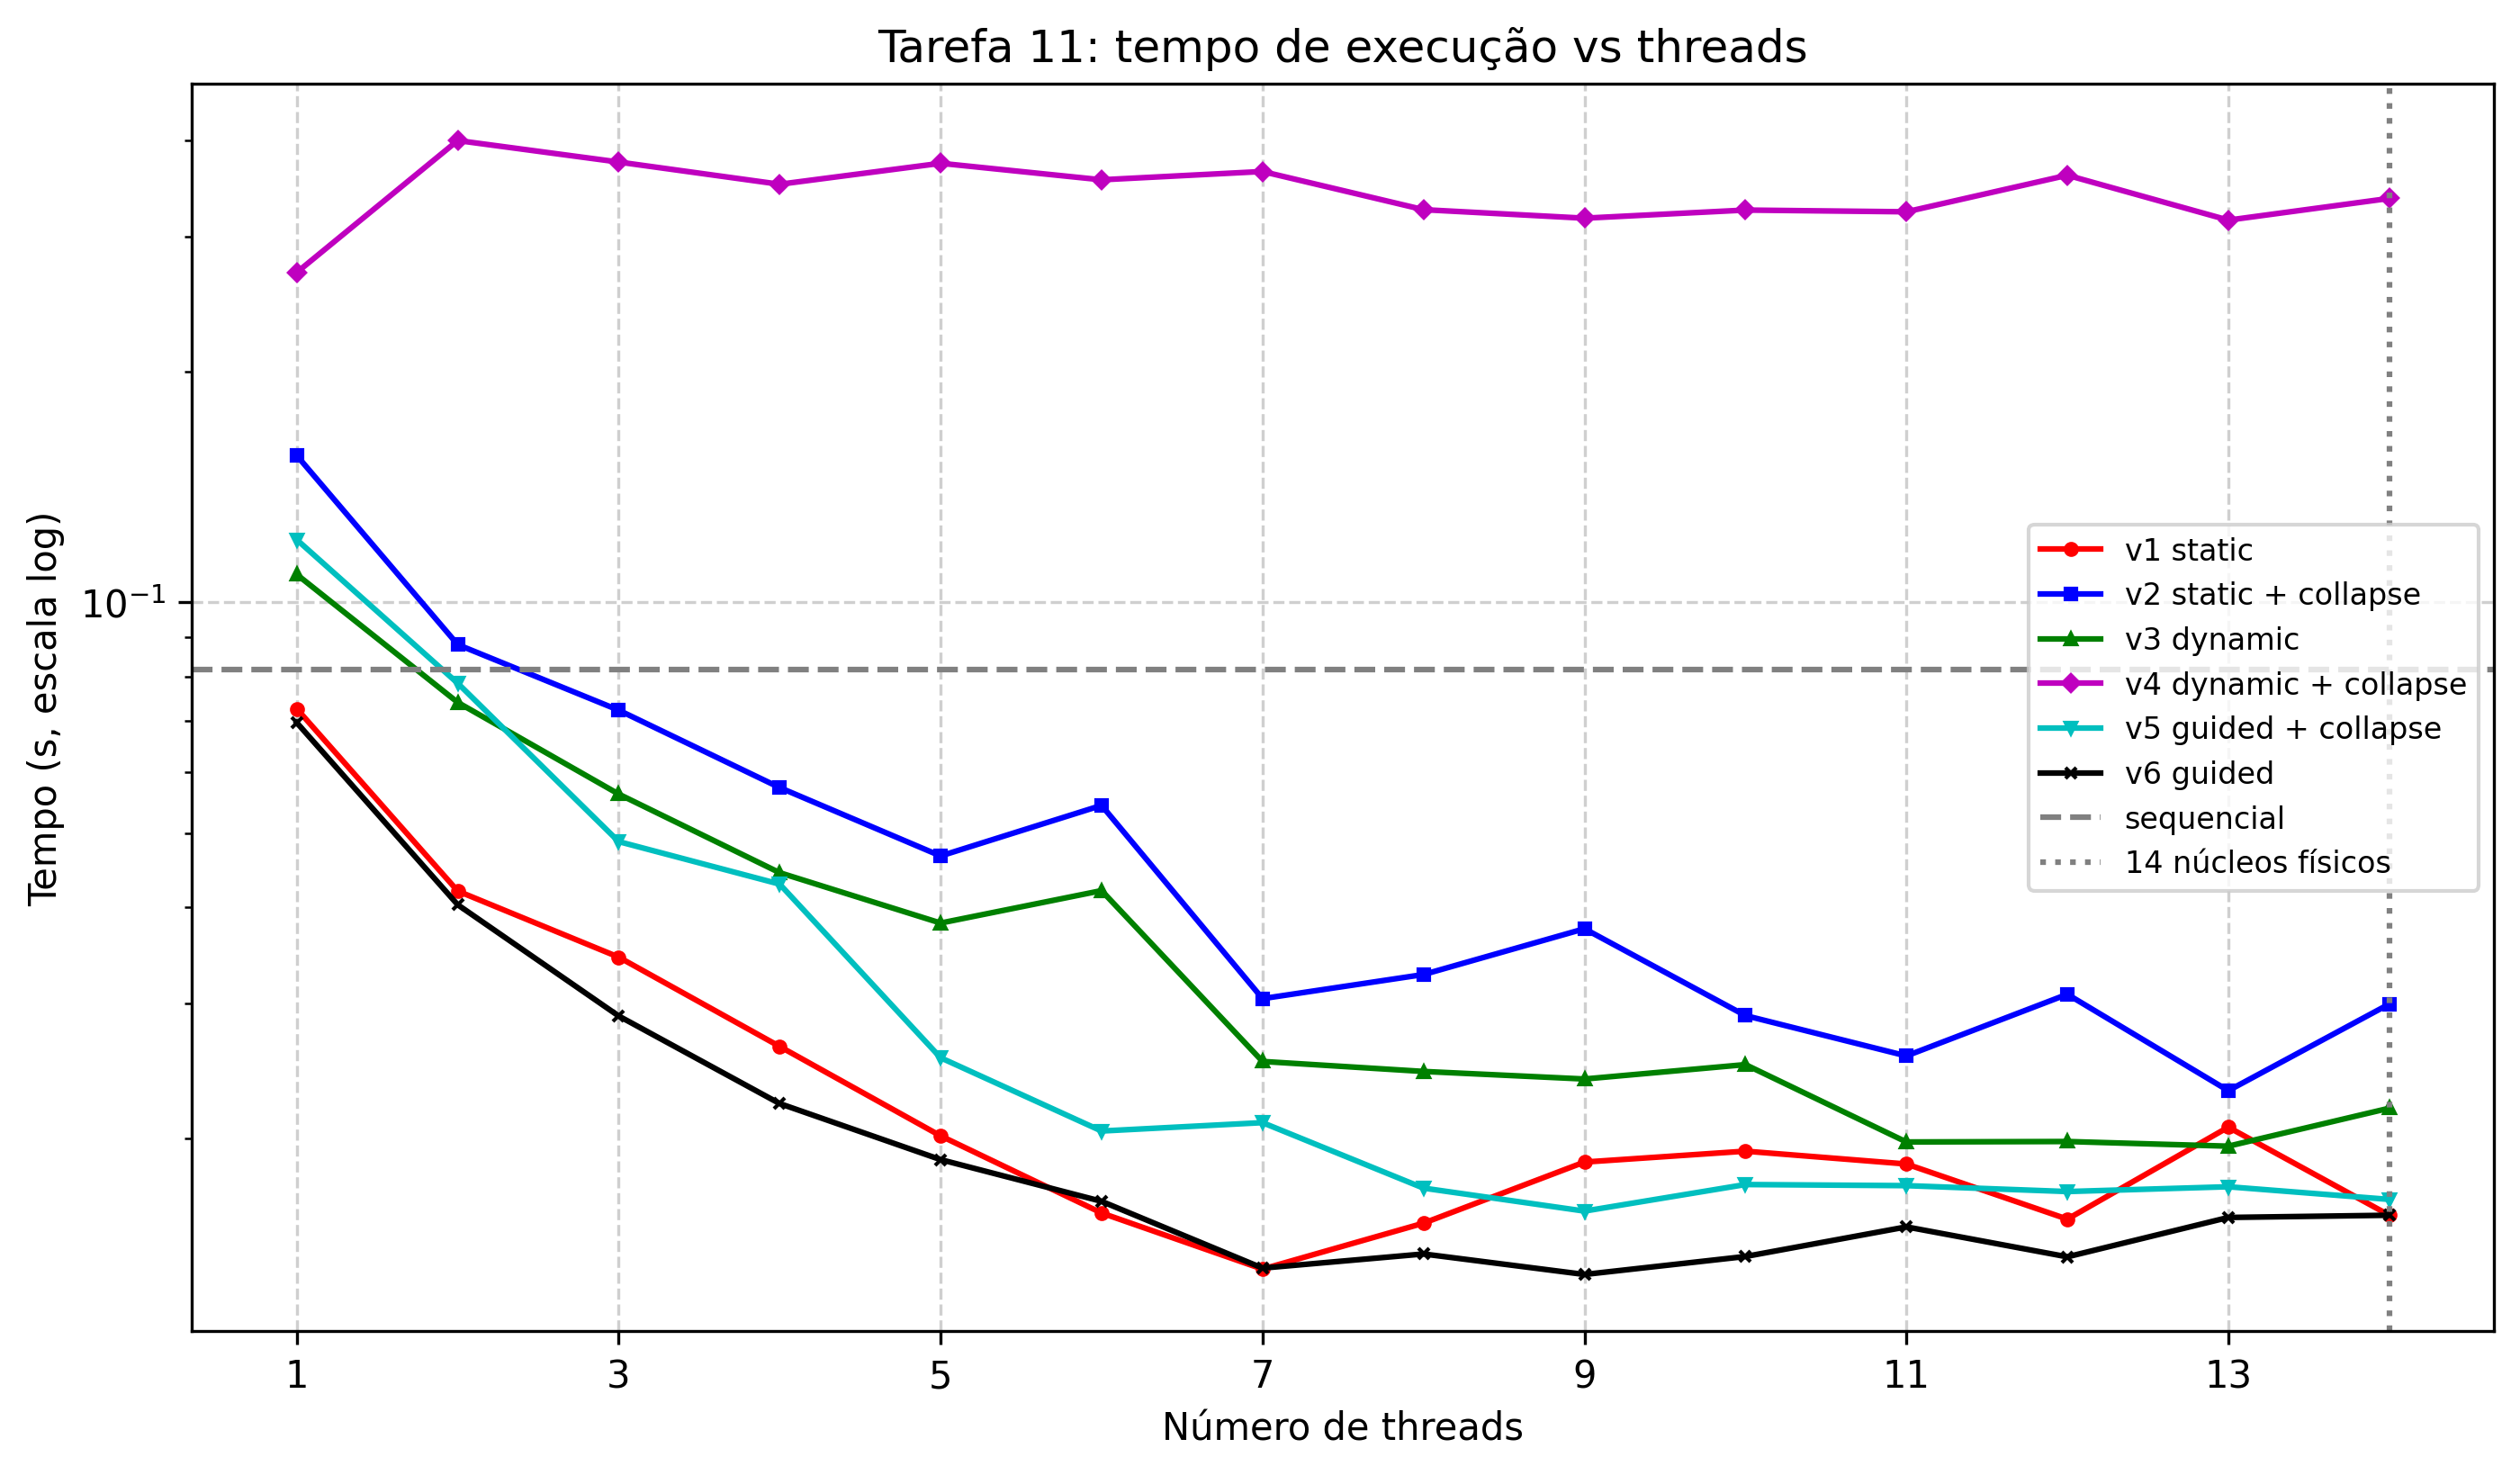
\includegraphics[width=0.98\textwidth]{../tempo_execucao_log_plot.png}
\caption{Tempo mediano das políticas com e sem \texttt{collapse(2)}, de 1 a 28 threads, em escala logarítmica.}
\label{fig:tempo}
\end{figure}

\begin{figure}[H]
\centering
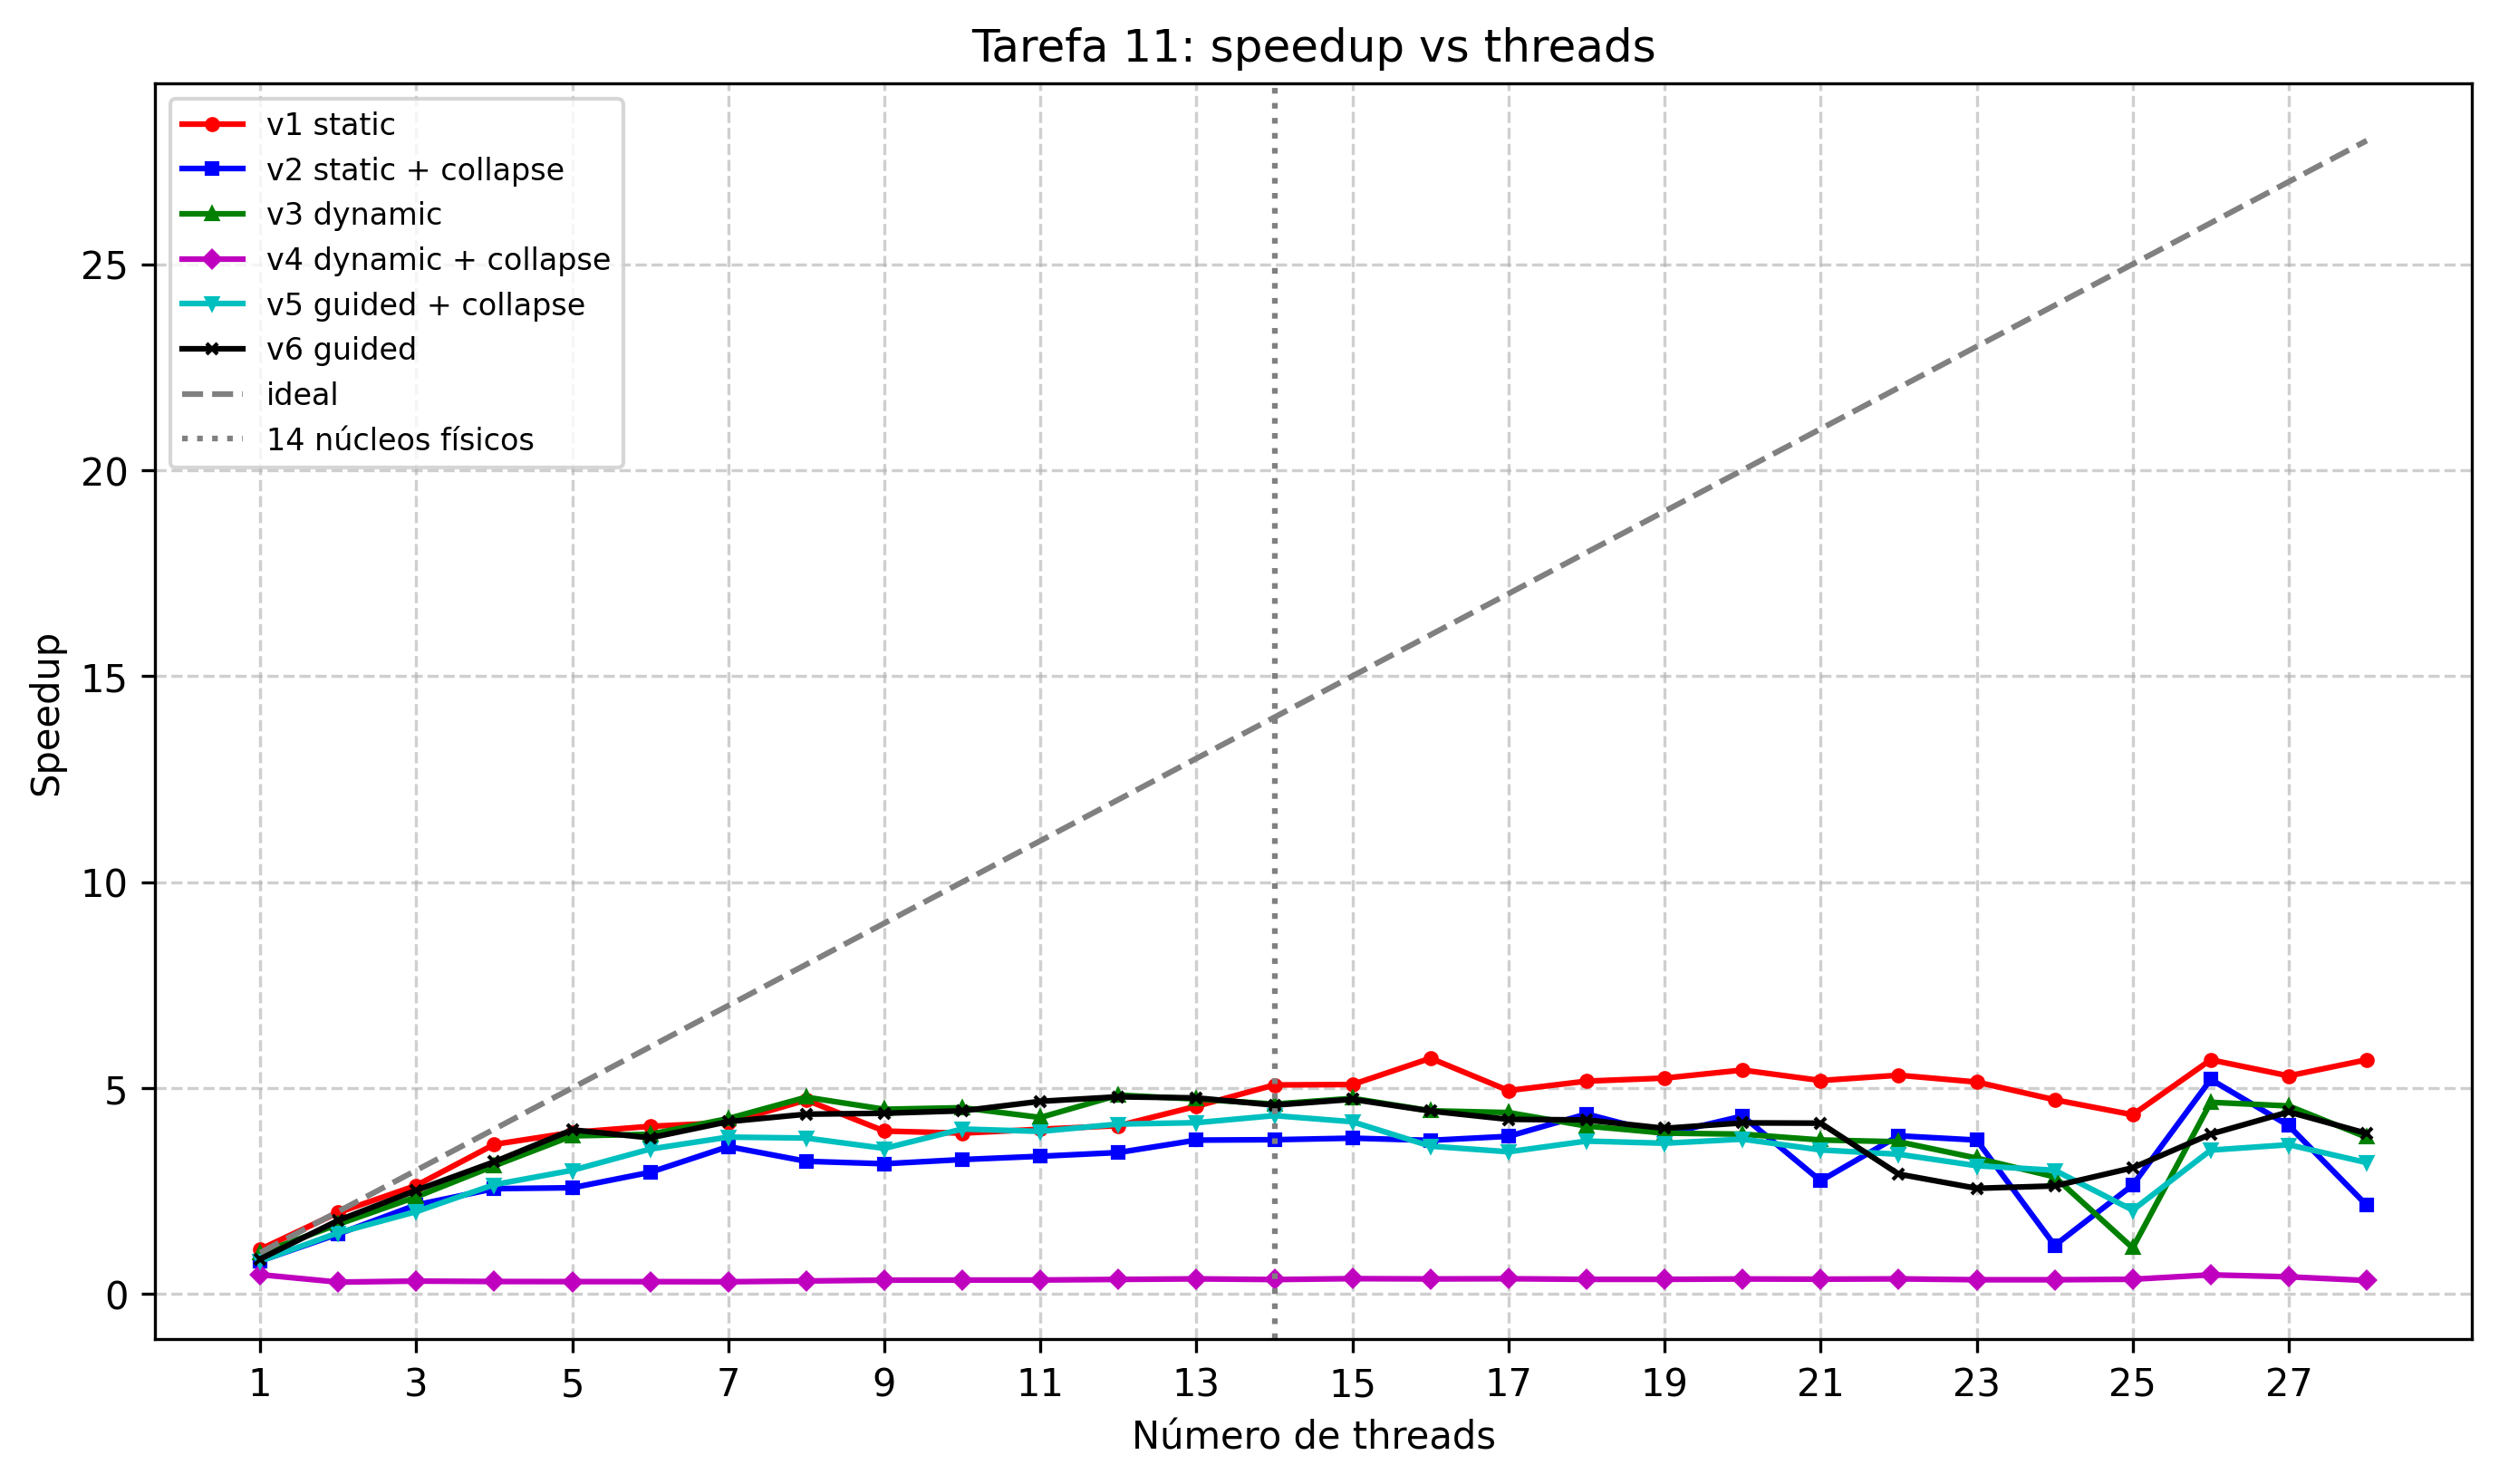
\includegraphics[width=0.98\textwidth]{../speedup_plot.png}
\caption{Speedup relativo à referência sequencial. A reta tracejada representa o caso ideal.}
\label{fig:speedup}
\end{figure}

\subsection{Variação do chunksize}
Para comparar as variantes com o mesmo volume de trabalho por chunk, foi realizado um segundo experimento com oito threads. Sem \texttt{collapse}, os chunks foram 1, 4, 16 e 64 linhas. Com \texttt{collapse}, foram utilizadas 510, 2.040, 8.160 e 32.640 células, quantidades equivalentes a 1, 4, 16 e 64 linhas internas. Cada configuração teve cinco repetições; os dados estão em \texttt{runs/chunks-20260911-152008-206654/}.

\begin{figure}[H]
\centering
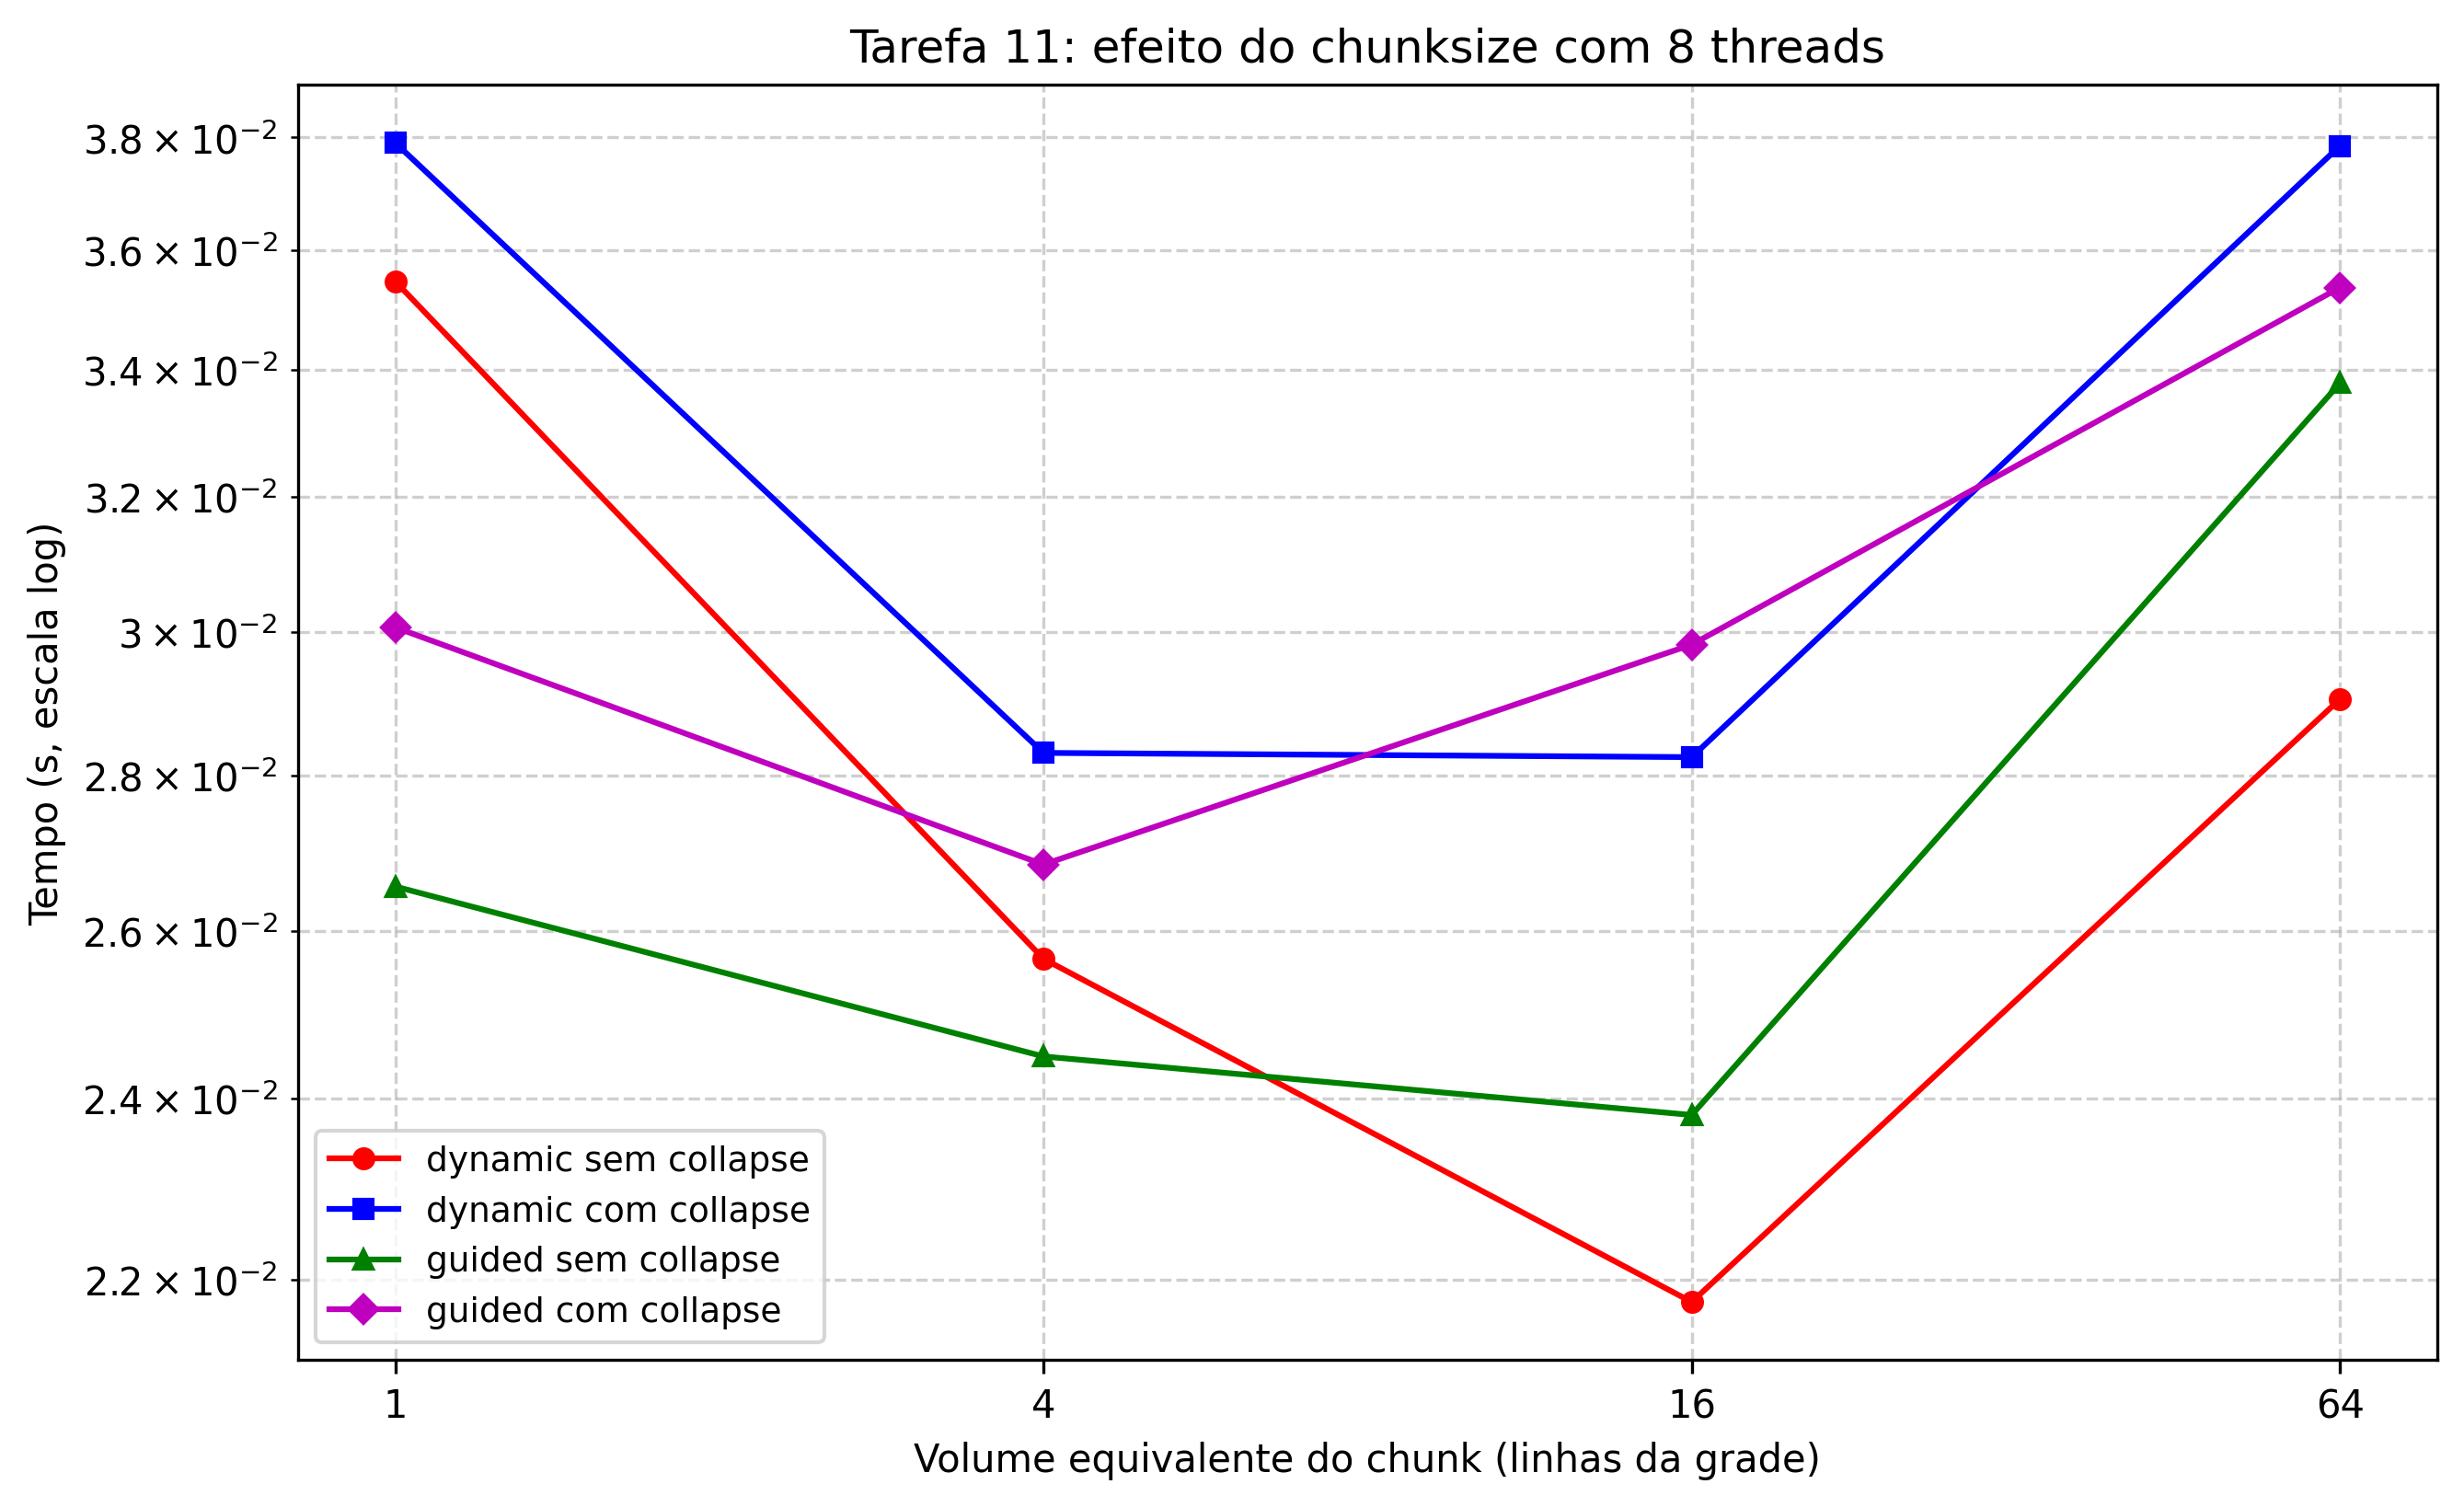
\includegraphics[width=0.92\textwidth]{chunksize_plot.png}
\caption{Efeito do chunksize com oito threads. O eixo horizontal representa o volume equivalente em linhas.}
\label{fig:chunks}
\end{figure}

No \texttt{dynamic}, o melhor resultado sem collapse ocorreu com 16 linhas por bloco (0,0218~s); com collapse, quatro e 16 linhas equivalentes ficaram próximos (0,0283~s). No \texttt{guided}, o menor tempo sem collapse ocorreu com mínimo de 16 linhas (0,0238~s); com collapse, o melhor mínimo foi de quatro linhas equivalentes (0,0268~s). Nos dois escalonamentos, o maior chunk testado, de 64 linhas equivalentes, foi mais lento que os tamanhos intermediários.
\section{Discussão}
\subsection{Granularidade e custo de distribuição}
A comparação entre v3 e v4 mostra por que o valor do chunk precisa ser interpretado junto com \texttt{collapse}. Com \texttt{dynamic,16}, o número de blocos por passo é:
\[
\text{sem collapse: }\left\lceil\frac{510}{16}\right\rceil=32,
\qquad
\text{com collapse: }\left\lceil\frac{260.100}{16}\right\rceil=16.257.
\]
No primeiro caso, um bloco completo reúne 8.160 atualizações; no segundo, apenas 16. Ao longo de 500 passos, são 16.000 e 8.128.500 blocos, respectivamente. Eles são unidades de distribuição do laço, e não novas threads.

Com quatro threads, v3 levou 0,0337~s e v4 levou 0,3482~s. A multiplicação dos blocos aumenta o trabalho de gerenciamento para a mesma quantidade de atualizações. O experimento com oito threads reforça essa interpretação: ao passar de 16 células para 8.160 células por chunk, a versão dynamic com collapse passou de 0,3342~s, na varredura principal, para 0,0283~s, no estudo de chunks. Assim, a piora de v4 está associada à granularidade adotada e não permite concluir que \texttt{collapse} seja sempre inadequado.

Em \texttt{guided}, o chunk é um mínimo e os blocos iniciais são maiores. Por isso, a contagem de blocos não segue a divisão fixa acima. Essa diferença ajuda a explicar por que v5 apresentou tempos menores que v4, embora ambas distribuam células.

\subsection{Localidade e limites de escalabilidade}
A versão v1, com \texttt{static} por linhas, obteve o menor tempo da varredura: 0,0183~s com 16 threads, contra 0,1049~s da referência sequencial. O speedup foi 5,72 e a eficiência, $E(p)=S(p)/p$, foi aproximadamente 35,8\%. Com quatro threads, o tempo foi 0,0289~s e o speedup foi 3,63.

A carga uniforme favorece a distribuição estática, que exige pouco gerenciamento. O acesso \texttt{c=i*N+j} percorre posições contíguas ao variar $j$ e permite reutilizar vizinhos no cache. Os menores tempos das versões dynamic e guided por linhas ocorreram com 12 threads: 0,0217~s e 0,0219~s, respectivamente.

Já existem 510 linhas internas para distribuir entre até 28 threads. Portanto, \texttt{collapse(2)} não é necessário para fornecer trabalho a toda a equipe nesta malha. Ele altera a granularidade e pode afetar os índices gerados e a vetorização. Esses efeitos individuais não foram medidos.

Os dois buffers ocupam 4~MiB. Em uma linha de cache de 64 bytes cabem oito valores \texttt{double}; escritas de threads distintas na mesma linha podem provocar falso compartilhamento. Entretanto, os tempos, isoladamente, não identificam esse efeito nem comprovam saturação da memória RAM. Parte dos dados pode ser reutilizada em cache.

Entre 16 e 28 threads, v1 apresentou pouca diferença nas medianas: 0,0183~s e 0,0185~s. O trabalho por thread diminui, mas as barreiras e o gerenciamento continuam presentes. Os picos da primeira varredura em 26--28 threads não se repetiram de forma sistemática na confirmação. A virtualização e o compartilhamento dos recursos de hardware também podem afetar os tempos; sua contribuição não foi isolada. Assim, 16 threads corresponde ao menor tempo medido, sem estabelecer uma quantidade ótima para outras malhas ou máquinas.

\section{Conclusão}
A implementação preservou os campos nulo e unitário e apresentou o espalhamento da perturbação gaussiana. Nos casos testados, as seis versões paralelas produziram campos idênticos ao da referência sequencial. A separação dos buffers e as barreiras entre atualização e troca de ponteiros mantêm a dependência entre os passos temporais.

Para a malha e o ambiente avaliados, \texttt{schedule(static)} sem \texttt{collapse} apresentou o menor tempo, com speedup de 5,72 em 16 threads. A versão \texttt{dynamic,16} com \texttt{collapse} teve os maiores tempos porque distribuiu blocos de apenas 16 células. O estudo com chunks equivalentes mostrou que aumentar esse volume reduz substancialmente o custo observado. Portanto, a escolha do escalonamento deve considerar o custo das iterações e a unidade de trabalho distribuída.

\appendix
\newpage
\section{Código-fonte}
O apêndice reúne os sete códigos completos utilizados nos testes e nas medições.
\lstinputlisting[caption={v0\_seq.c: referência sequencial}]{../v0_seq.c}
\newpage
\lstinputlisting[caption={v1\_static.c: static por linhas}]{../v1_static.c}
\newpage
\lstinputlisting[caption={v2\_static\_collapse.c: static por células}]{../v2_static_collapse.c}
\newpage
\lstinputlisting[caption={v3\_dynamic.c: dynamic por linhas}]{../v3_dynamic.c}
\newpage
\lstinputlisting[caption={v4\_dynamic\_collapse.c: dynamic por células}]{../v4_dynamic_collapse.c}
\newpage
\lstinputlisting[caption={v5\_guided\_collapse.c: guided por células}]{../v5_guided_collapse.c}
\newpage
\lstinputlisting[caption={v6\_guided.c: guided por linhas}]{../v6_guided.c}
\end{document}
